\documentclass[a4j]{jarticle}

\usepackage{amsmath,amssymb,bm}
\usepackage{caption}
\usepackage{minitoc}
\usepackage{hhline}
\usepackage{algorithmic}
\usepackage{algorithm}
\usepackage{booktabs}
\usepackage[dvipdfmx]{graphicx} 
\usepackage[dvipdfmx, usenames]{color}
\usepackage{colortbl}
\usepackage{ascmac}
\usepackage{lscape}
\usepackage{url}
\usepackage{graphicx}
\usepackage{float}
\usepackage{siunitx}
\usepackage{subfig}
\usepackage{comment} 

\addtolength{\topmargin}{-2cm}
\addtolength{\textheight}{4cm}
\addtolength{\textwidth}{2cm}
\addtolength{\oddsidemargin}{-1cm}
\addtolength{\evensidemargin}{-1cm}


\begin{document}

\twocolumn[
\begin{center}
	{\Large タイコグラフィ法による大型X線ウォルターミラーの光学的評価}
\end{center}
\begin{center}
	{\Large Large }
\end{center}

\begin{flushright}
	{\large 03-190395 渡辺 貴史} \\ % author
	{\large 指導教員 三村 秀和 准教授} % teacher
\end{flushright}

\begin{center}
 {\bfseries 概要}
\end{center}

太陽の構造や活動について未解明の現象が多く存在する。
FOXSI4プロジェクトでは、太陽コロナの高温プラズマが発するX線領域の電磁波を計測することで、これらを明らかにすることを1つの目標としている。
FOXSI4に搭載予定のWolter I型のミラーについて、秒角分解能の向上のためには加工プロセスの改善が必要であり、結像性能の悪化要因を特定できる測定装置が必要である。
測定装置は、ミラー内面を傷つけない非接触式であり、かつ素早く計測できる簡素なものが好ましい。
これを満たす波面計測法の中でも、Wolterミラーの細い輪帯の測定に適している位相回復法を採用し、新たな実験系を提案した。
実際に加工されたWolterミラーの計測実験を行った。
\vspace*{2em}
]
%\thispagestyle{empty}

\section{序論}
天文分野において太陽の活動を観測することは非常に重要である。
2023年に打ち上げ予定のFOXSI4プロジェクトでは、太陽コロナの活発な領域において高温プラズマが発するX線領域の電磁波を計測することで、これらを明らかにすることを1つの目標としている。
FOXSI4に搭載予定のWolter I型のミラーについて、解像分解能の向上のためには加工プロセスの改善が必要であり、結像性能の悪化要因を特定できる測定装置が必要である。
測定装置は、ミラー内面を傷つけない非接触式であり、かつ素早く加工プロセスにフィードバックできる簡素なものが好ましい。
また、受光面積を大きくするため複数枚のWolterミラーをネスト構造にしたNested Wolterミラーに対しても適用可能な系であることが求められる。
これを満たす計測法として波面計測法があり、中でも特にWolterミラーの非常に細い輪帯を測定できる高分解能な測定が可能である位相回復法を採用する。

口径が大きく射入射角の小さいWolterミラーはNAがやや低く、計測するべき波面は図\ref{fig:wolter_thinring}に示すように非常に細い輪帯状になる。
輪帯の幅(外円と内円の半径の差)は設計形状に対して\SI{363.3}{\micro \metre}であり、波面計測に求められる空間分解能は非常に高いものとなる。
波面精度を十分に確保しつつ、空間分解能が十分に高い波面計測法を開発する必要がある。

\begin{figure}[h!]
\centering
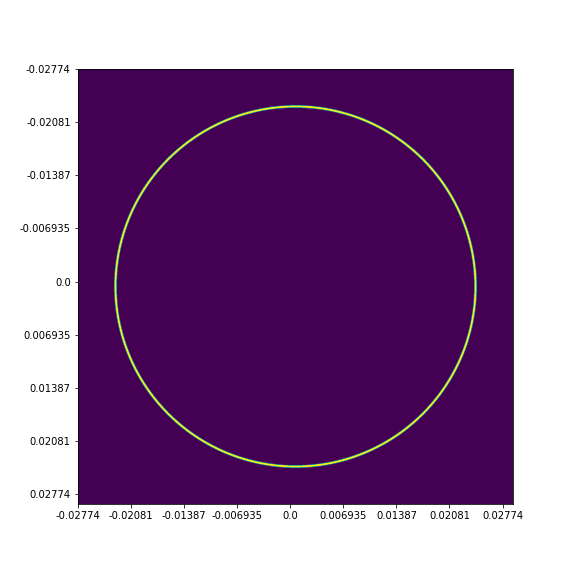
\includegraphics[width=7cm]{../thesis/chap1/figure/wolter_thinring.png}
\caption{Wolterミラー下流端面における集光波面}
\label{fig:wolter_thinring}
\end{figure}

\section{手法の検討}

位相回復法とは、測定対象のミラーによって集光されたビームに位相物体を差し入れ、背後に現れる回折像の強度分布計測値から繰り返し計算によって位相情報を算出する方法である。
素子の最小サイズによる律速がないため、測定する際の配置を工夫することで非常に高い空間分解能が実現できる。
位相回復法の系として幾つかの種類が考えられる。
焦点面でオブジェクトを走査する方法では、ミラー下流端面における空間分解能を十分確保するために必要な走査回数が数千回となってしまい、計測時間として現実的ではない。

\subsection{下流端開口走査による冗長性}
\label{chap3_transverse_introduction}

オブジェクトを走査する位置を焦点面ではなく集光素子の開口直後とするTransverse Translation法がBradyらによって提案されている。\cite{Brady2009}
これは図\ref{fig:transverse_schematic}に示すように、焦点面を操作するタイコグラフィ法同様に穴の空いたピンホールオブジェクトを集光素子の開口で走査し、その回折像を下流側のカメラで撮影するという方法である。
この方法は、焦点面において1枚だけ強度分布を取得し位相回復計算を行う場合に比べ、ピンホールによりNAが低下し、メインピークが下がるためダイナミックレンジの観点から有利である。

\begin{figure}[!ht]
\centering
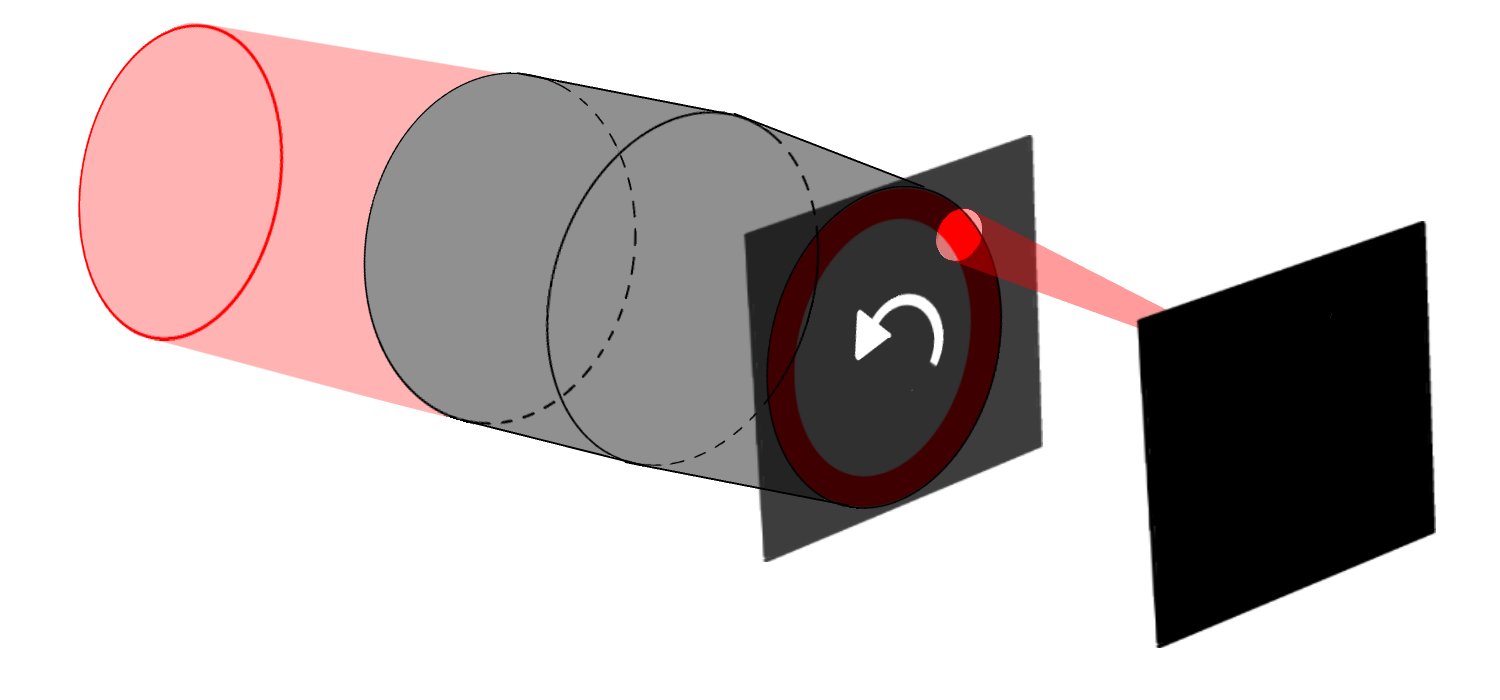
\includegraphics[width=6cm]{../thesis/chap3/figure/transverse_schematic.png}
\caption{Transverse Translation Diversityの概要}
\label{fig:transverse_schematic}
\end{figure}

\begin{figure}[!ht]
\centering
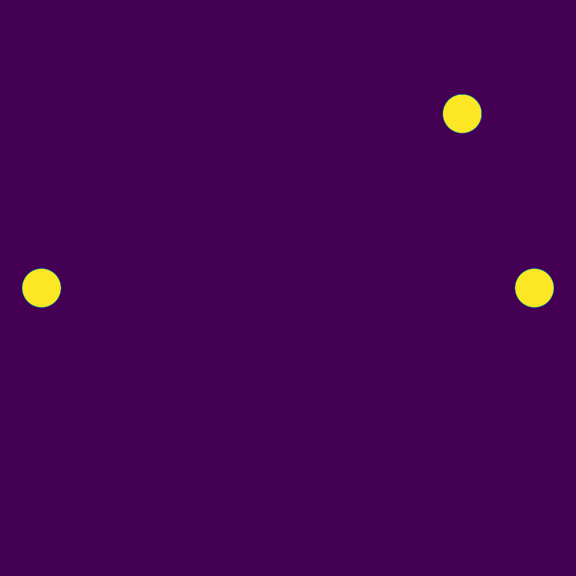
\includegraphics[width=5cm]{../thesis/chap3/figure/three_pinhole_mask.png}
\caption{3つ穴ピンホールの設計}
\label{fig:transverse_schematic}
\end{figure}

しかし、ビームの対称性から、ピンホールが1つでは位相回復計算が収束しない。
これを解決するため、穴を3つ不等間隔で開けたオブジェクトを用いて走査する方法を提案する。
シミュレーションの検討により、不等間隔の3つ穴を持つピンホールオブジェクトによる位相回復計算が収束することを確認した。

\section{ミラー計測実験}

ミラーに合わせて実験装置を設計した。
ピンホールは自動回転ステージに取り付けられ、ミラー下流端直後に配置された。
ミラーの置き直しに対する再現性を高めるため、ミラーに合わせて把持機構を設計した。

\begin{figure}[!ht]
\centering
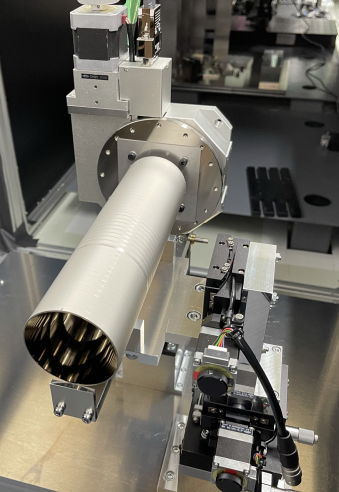
\includegraphics[width=5cm]{../thesis/chap5/figure/photo_mirror_pinhole.png}
\caption{ミラー測定実験系 写真}
\label{fig:photo_mirror_experiment_mirror_and_pinhole}
\end{figure}

2021年1月に三村グループによって作製されたWolterミラーに対して提案手法を適用し、測定実験を行った。

\begin{figure}[!ht]
\centering

\includegraphics[width=5cm]{../thesis/chap5/figure/reconstructed_phase_unwrapped.png}
\caption{回復された位相分布}
\label{fig:reconstructed_phase_unwrapped}
\end{figure}

\begin{figure}[!ht]
\centering
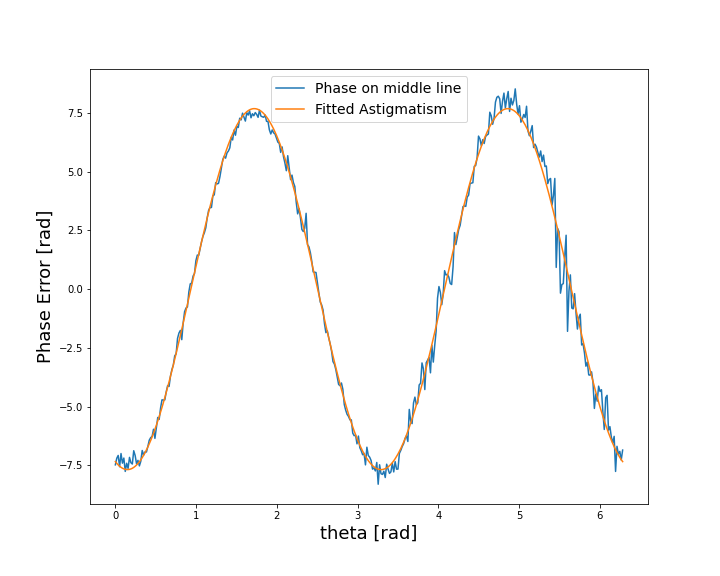
\includegraphics[width=5cm]{../thesis/chap5/figure/astigmatism_fitted.png}
\caption{フィッティングされた非点収差成分}
\label{fig:astigmatism_fitted}
\end{figure}

位相回復結果から焦点面での強度分布を再構成したところ、撮影された焦点面の強度分布と良く一致した。
このことから、位相回復計算の妥当性が確認できた。

非点収差成分は周方向誤差に換算すると\SI{101.5}{\micro \metre}となった。
これは真円度測定データと矛盾するため、ミラーではなく上流の光学系による非点収差が原因ではないかと考えた。
ミラーを光軸方向周りに回転させたところ、焦点面における非点収差由来の模様は回転せず、その場に留まった。
このことから、ミラーではなく上流光学系由来の非点収差であると結論づけた。
理想的なレンズを用いた実験によって上流光学系を校正した上で、再度実験を行うことで、ミラーに起因する波面誤差が計測できると考えられる。

\bibliography{references}
\bibliographystyle{siam}

\end{document}